
\section{measurements model}

acceleration data from imu \\
magnetic field orientation vector \\
RSSI

% Consider the process is Markovian.

\section{Transition model definition}

Copied all from \cite{articleXia}:

With  the  development  of  microelectromechanical  systems(MEMS),  a  few  MEMS-based  sensors  have  been  built  and
incorporated  into  smartphones:  accelerometers,  gyroscopes,magnetometers,  etc.  These  sensors  can  be  used  to  provide information  on  the  user’s  actions.  Pedestrian  dead  reckon-ing  (PDR)  [10]  is  a  relative  navigation  technique  that  uses these sensors.

we propose a PDR-based  indoor positioningmethod  that  integrates  RSSI  with  indoor  environment  mapconstraints by using particle filters.

PDR-based indoor positioning can be expressed by the following equations

\begin{equation}
X_k = \
\begin{bmatrix} 
x_{t-1} \\
y_{t-1} 
\end{bmatrix} = \
\begin{bmatrix} 
x_{t-1} &+ l_k \sin(\theta_t) \\
y_{t-1} &+ l_k \cos(\theta_t) 
\end{bmatrix} + \
\begin{bmatrix} 
\delta_{x} \\
\delta_{y} 
\end{bmatrix}
\end{equation}

The orientation  updates is independent from $X_k$ updates, depends on accelerometer and gyro, same model.

Step   Detection:Android   mobile   phones   have   two kinds  of  sensors  to  monitor  steps:  step  counters  and  step detectors [25]. 

Peak detection is used in this paper for step detection

nonlinear step length estimation model based on statistics proposed by Weinberg [27]

\begin{equation}
s = k \sqrt[4]{a_{z max} - a_{z min}}
\end{equation}

The Android system computes orientation angles by using the  device’s  geomagnetic  sensors  in  combination  with  its accelerometers   [25].   Using   these   two   hardware   sensors,the  system  provides  data  for  the  following  three  orientation angles

The  device is NOT  assumed to  be pointing in the heading direction. Need to apply additional space transformation.

\subsection{RSSI methode}

Usual path-loss model:

\begin{equation}
PL(d) = PL(d0) + 10 \alpha \log{d / d_0} + \omega = 
PL(d0) + 10 \alpha \log{d / d_0} + N(0, \sigma^2_{\omega})
\end{equation}

where $d$ represents the Euclidean distance between the anchor node  and  the  receiver,d0represents  a  specified  distance,PL(d)and PL(d0)represent the RSSI at $d$ and $d_0$, respectively(in  dBm),  and $\alpha$ represents the  path  loss  exponent, which  is closely related to the ambient environment; $\omega$ is a zero-mean Gaussian distribution variable with variance $\sigma^2_{\omega}$.

The inverse function: 
\begin{equation}
d_i = d_0 \cdot 10 \frac{PL(d_i) - PL(d_0)}{10\alpha}
\end{equation}

Landmark model:

\begin{align}
f_i(x, y) &= d_i - \sqrt{(x - x_i)^2 + (y - y_i)^2} \\
min(x, y) &= min \sum_{i=1}^{m}[f_i(x, y)]^2, m \ge 3.
\end{align}

In paper author transform this to linear system, 

\begin{align}
AZ & = b \\
A &= \begin{bmatrix} 
1 - 2 x_1 - 2 y_1 \\
... \\
1 - 2 x_m - 2 y_m
\end{bmatrix} \\
Z &= \begin{bmatrix} 
x^2 + y^2 \\
x \\
y
\end{bmatrix} \\
b &= \begin{bmatrix} 
d_1^2 - x_1^2 - y_2^2\\
...\\
...
\end{bmatrix}
\end{align}

We have to check it

Good alternative was proposed in \cite{} to bound region by min and max RSSI according to its variance - linear system.

\subsection{Processing}

Update step, prediction, correction
State Estimation


Resample:In  this  step,  importance  resampling  [20]  isused to obtain a new particle set

some papers prove importance resampling can't be applied for this task because pf noise.
% observation equation:

% \section{Crasy Idea}

% There is some similarity in video compressing process

% We strore gradients of changing signal measurements, we apply searching procedure to have a smooth measurements.

% We have a convex magnetic field and a trajectory, 
% the task is to find similar trajectrory with highest correlation to measurements.

% Regression, approximation, pattern matching, Convolutions.

% Gradients, blockmatching

% Different approaches in papers, play on a toy model.


\subsection{RSSI Graph SLAM}

Definition taken from \cite{7809951}.

Trajectory Modeling with GraphSLAM\cite{SLAM_using_Gaussian_process_latent_variable_models}   is   a   classical   framework   for SLAM optimization.

GraphSLAM  extends  the  traditional  SLAM  framework  by considering  the  poses  in  a  trajectory  as  nodes  and  raw  measurements between poses and landmarks as edges in a graph.Note that each edge is attached with a probability distribution over  the  relative  positions  of  its  two  vertexes  since  inherent noise in sensors need to be considered. In 2-D case, a pose $x_t$ consists of a 2-D coordinates $(x_1,t,x_2,t)$ and an yaw angle $\theta_t$.

\begin{equation}
e_{i j}(x_i, x_j) = z_{i j} - \hat z_{i j} (x_i,x_j)
\end{equation}

The item $\omega_{i j}$ in the equation is the information matrix representing Gaussian noise in sensor measurement.The GraphSLAM problem is now reduced to a constrained least  square  problem  and  it  can  be  solved  by  some  standard optimization techniques, like Gaussian-Newton or Levenberg-Marquardt algorithms, as proposed in [16]. Either of the two methods is based on local iterative linearization: 
%x′=  ̆x+ ∆x

Then,  the  goal  of  GraphSLAM  is  to  find  an  configuration of  poses $x^{*}$ that  minimizes  the  squared  error F(x) of  all observations given a set of constraint edges C:

\begin{align}
F(X) =\sum_{(i,j)\in C} e_{i j}^T Ω_{ i j} e_{i j} \\
x^{*} = argmin_x F(x)
\end{align}


\section{Experiments}

\subsection{Pose estimation and IMU Modelling}

\begin{figure}
	\centering
	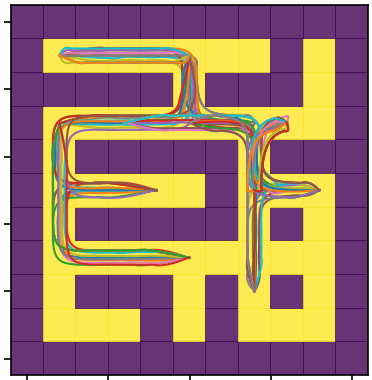
\includegraphics[width=0.4\linewidth]{images/routes2}
	\caption{Random trajectories on a generated building map.}
	\label{fig:routes1}
\end{figure}

We generate the series of data using maze generation algorithm. On a fixed map of corridors we generate routes and trajectories, then we add noise to simulate the walking human.

\begin{figure}
	\centering
	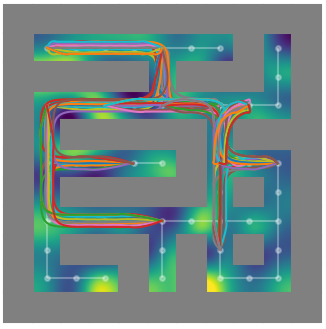
\includegraphics[width=0.4\linewidth]{images/routes3}
	\caption{The background simulates continuous random field we want to reconstruct}
	\label{fig:routes3}
\end{figure}

\subsection{Data processing}

First we focus on a key part of a given research. The main part of this paper requires the transformation of observation to the solid continious map.

After we highlighted the map structure and features, we can say that we need to reconstruct the magnetic field.

A magnetic field is continious potential field with certain known features. Each point has its own field direction and magnitude.
We can encode the field as a number of three dimensional vectors or as 3 images, representing the field magnitude in each axis direction.

First we model the field construction and reconstruction. 

\subsubsection{image approximation}

We generate a surface from array with random noise values as a mesh and apply interpolation and smoothing.
On the random surface we sample a series of points. The problem is to accurately reconstruct the initial surface from samples.

There are  several possible solutions for such problem. The most promising and accurate seems kernel training as in Kernel Ridge Regression or other similar methods. From the other side, there are other more straightforward solutions.

Solution 1: interpolation. Solution is not accurate and not feasible because resulting surface is very noisy. We need a solution to deal with many observations and noisy data.

The promising solution was shown in repository of \cite{Surface_approximation_GP}. We aim to solve the problem in similar problem statement with more traditional methods.

\begin{figure}
	\centering
	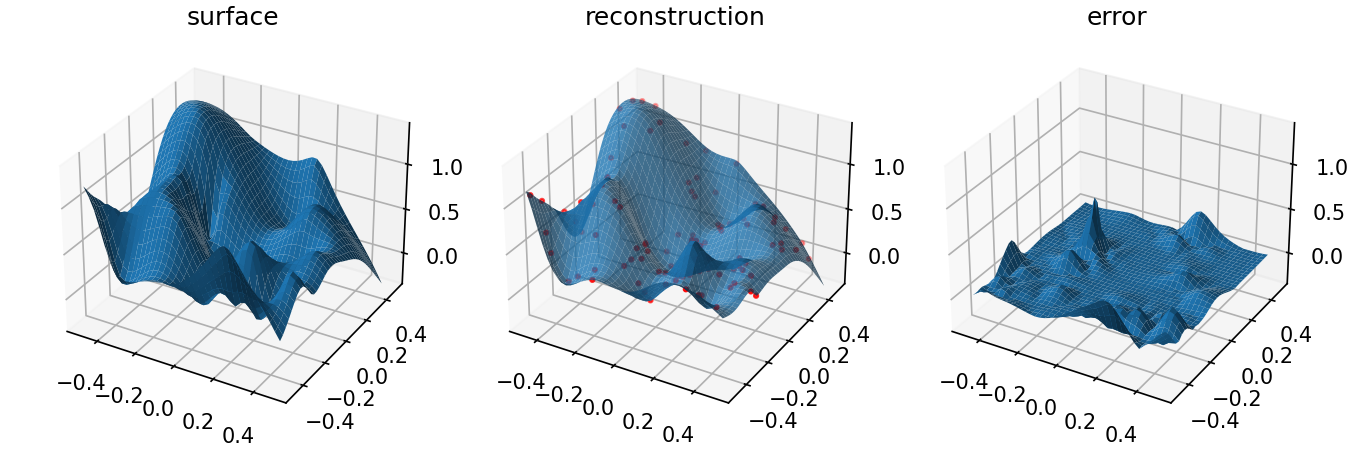
\includegraphics[width=1.0\linewidth]{images/rbfinterp3d}
	\caption{}
	\label{fig:rbfinterp3d}
\end{figure}

We perform the noisy surface approximation using RBF function from the scipy package.

On the figure \ref{rbfinterp3d}, the right plot represents the distance between initial and approximated surfaces.